\documentclass[conference]{IEEEtran}
\usepackage{graphicx}
\usepackage{amsmath}
\usepackage{cite}
\usepackage{amsfonts}
\usepackage{algorithmic}
\usepackage{array}
\usepackage{booktabs}
\usepackage{url}
\usepackage{subcaption}
\usepackage{placeins}
\usepackage{flushend}

\begin{document}

\title{Temperature-Dependent Temporal Scaling for Physics-Informed Neural Network in Battery State-of-Health Estimation}

\author{
\IEEEauthorblockN{S. H. Ellahie, M. A. Faisal}

\IEEEauthorblockA{
Ghulam Ishaq Khan Institute of Engineering Sciences and Technology\\
Topi, Pakistan\\
Email: u2024545@giki.edu.pk, u2024335@giki.edu.pk
}
}

\maketitle
    
\begin{abstract}
Accurate state-of-health (SOH) estimation is essential for the safe and reliable operation of lithium-ion batteries. SOH is defined as the ratio of current capacity to nominal capacity, with end-of-life typically set at 80\%. Physics-informed neural networks (PINNs) have recently emerged as a powerful method that combines data based predictions with knowledge of how batteries age. However, most existing PINN-based approaches treat the cycle number as a linear measure of aging while ignoring the effect of temperature on the rate of degradation. In this work, we introduce a simple yet effective modification: scaling the cycle number using the Arrhenius equation to account for the effect of temperature on the aging time. This transformation is embedded directly into the PINN forward pass as a learnable activation energy parameter. We validate our approach on the TJU NCA battery dataset, which includes cells cycled at 25\textdegree C, 35\textdegree C, and 45\textdegree C. Training is performed on 25\textdegree C and 45\textdegree C data, with 35\textdegree C held out for testing. Compared to a standard PINN without temperature scaling, our proposed Arrhenius-scaling PINN reduces the holdout test MSE from 5986.26 to 674.26~mA\textsuperscript{2}\textperiodcentered h\textsuperscript{2} (an 88.7\% reduction) and improves the R\textsuperscript{2} from $-1.760$ to $0.689$. On the in-distribution random split, the proposed model improves R\textsuperscript{2} from 0.953 to 0.980 and reduces MSE by 57.8\%. The learnable activation energy converges to approximately 48.5~kJ/mol, which is consistent with reported growth kinetics of the solid-electrolyte interphase (SEI). These results indicate that incorporating Arrhenius temporal scaling can improve the robustness and generalization capability of PINN-based battery prognostics.
\end{abstract}

\section{Introduction}
Lithium-ion batteries are widely used in portable electronics, electric vehicles, and large-scale energy storage systems because they offer high energy density and long service life. Over time, however, batteries gradually lose their ability to store energy due to capacity degradation and increasing internal resistance. Accurately estimating the battery's state-of-health (SOH), which represents the remaining capacity relative to its original rated capacity, is important for battery management systems (BMS). Reliable SOH estimation helps ensure safe operation, improve charging control, and predict the battery's remaining useful life. In most applications, a battery is considered to have reached its end-of-life when its SOH decreases to 80\% of its original capacity.

Temperature is one of the most critical factors accelerating battery aging. Elevated temperatures promote solid-electrolyte interface (SEI) growth, solvent decomposition, and other side reactions, leading to faster capacity loss~\cite{spotnitz2003,bloom2005}. The Arrhenius equation describes this temperature dependence quantitatively, stating that reaction rates increase exponentially with temperature. While many empirical and semi-empirical aging models incorporate Arrhenius terms, they are often chemistry-specific and require extensive parameter tuning.

In recent years, data based approaches like the Gaussian processes, random forests, and deep neural networks have shown impressive results in SOH estimation~\cite{severson2019}. However, pure black-box models may lack physical consistency and extrapolate poorly outside their training set. Physics-informed neural networks (PINNs)~\cite{raissi2019physics} offer a compelling alternative by embedding differential equations that govern degradation dynamics into the loss function. Wang et al.~\cite{wang2024physics} successfully applied PINNs to battery SOH estimation, achieving superior predictive accuracy and stability across multiple datasets. Nevertheless, their formulation treats cycle number as a raw linear time index, thereby ignoring the profound influence of temperature on aging kinetics.

To address this limitation, we introduce a physically motivated temporal scaling mechanism that explicitly accounts for temperature-dependent aging behavior. We replace the raw cycle number with an equivalent aging time computed via the Arrhenius equation, where the activation energy is treated as a learnable parameter. This simple modification allows the PINN to automatically discover the temperature acceleration factor from data while maintaining the original architecture. We demonstrate that the proposed method improves both in-distribution fit and out-of-distribution generalization to an unseen temperature (35\textdegree C) on the TJU NCA dataset.

\section{Methodology}
\subsection{Dataset and Feature Description}
We use the publicly available Tianjin University (TJU) lithium-ion battery dataset~\cite{zhu2022data}, which comprises commercial nickel-cobalt-aluminum oxide (NCA) cells cycled under constant-current constant-voltage (CC-CV) charging protocols at three constant temperatures: 25\textdegree C, 35\textdegree C, and 45\textdegree C.

We evaluate our approach under two protocols:
\begin{enumerate}
    \item \textbf{In-distribution (random split):} All cells from all three temperatures are randomly split into training and testing sets. This evaluates the model's ability to learn temperature-dependent aging patterns when data from all temperatures are available during training.
    \item \textbf{Out-of-distribution (holdout temperature):} Cells at 35\textdegree C are completely held out as the test set. Training uses only cells from 25\textdegree C and 45\textdegree C (with a random split within those two temperatures for training/validation). This tests cross-temperature generalization to an unseen intermediate temperature.
\end{enumerate}

Sixteen statistical features are extracted from each CC-CV charging cycle, capturing both the voltage and current profiles as well as time-based and derivative-based signatures. Table~\ref{tab:features} lists these features, which together capture degradation trends and cycle-to-cycle anomalies. All features are normalized using min-max scaling to the range \([-1, 1]\), and the SOH target (capacity in mA\textperiodcentered h) is normalized to \([0, 1]\).

\begin{table}[htbp]
\centering
\caption{Statistical features extracted from CC-CV charging windows}
\label{tab:features}
\begin{tabular}{@{\hspace{1em}} l c @{\hspace{1em}}}
\toprule
\textbf{Feature} & \textbf{Window} \\
\midrule
Mean                         & Voltage \\
Standard deviation           & Voltage \\
Skewness                     & Voltage \\
Kurtosis                     & Voltage \\
Charging time                & Voltage \\
Accumulated charge           & Voltage \\
Slope ($dV/dt$)              & Voltage \\
Entropy                      & Voltage \\
\midrule
Mean                         & Current \\
Standard deviation           & Current \\
Skewness                     & Current \\
Kurtosis                     & Current \\
Charging time                & Current \\
Accumulated charge           & Current \\
Slope ($dI/dt$)              & Current \\
Entropy                      & Current \\
\bottomrule
\end{tabular}
\end{table}

\subsection{Baseline PINN without Temperature Scaling}
The baseline PINN follows the architecture of Wang et al.~\cite{wang2024physics} and consists of two sub-networks:
\begin{itemize}
    \item \textbf{Solution network} \(\mathcal{F}(t, \mathbf{x})\): Maps the normalized cycle time \(t = k/100\) (where \(k\) is the cycle number) and feature vector \(\mathbf{x} \in \mathbb{R}^{16}\) to the SOH \(u\). The encoder consists of two hidden layers of 60 neurons each with \(\sin\) activation and dropout (\(p=0.2\)), projecting to a 32-dimensional representation. The predictor maps this representation through one hidden layer of 32 neurons (\(\sin\) activation) to a single output neuron. Total input dimension: 17 (1 time + 16 features).
    \item \textbf{Dynamics network} \(\mathcal{G}(t, \mathbf{x}, u, \partial u / \partial t, \nabla_{\mathbf{x}} u)\): Models the degradation dynamics. It takes as input the time \(t\), the features \(\mathbf{x}\), the predicted SOH \(u\), the temporal derivative \(\partial u / \partial t\), and the feature-space gradient \(\nabla_{\mathbf{x}} u \in \mathbb{R}^{16}\). The network is an MLP with two hidden layers of 60 neurons each (\(\sin\) activation) with dropout (\(p=0.2\)) and one output neuron. Total input dimension: 35 (1 + 16 + 1 + 1 + 16).
\end{itemize}
Both networks use Xavier normal initialization. The training loss is a weighted sum:
\[
\mathcal{L} = \mathcal{L}_{\text{data}} + \alpha \mathcal{L}_{\text{PDE}} + \beta \mathcal{L}_{\text{mono}},
\]
where
\begin{itemize}
    \item \(\mathcal{L}_{\text{data}} = \text{MSE}(u_{\text{pred}}, u_{\text{true}})\),
    \item \(\mathcal{L}_{\text{PDE}} = \text{MSE}\left(\frac{\partial \mathcal{F}}{\partial t}, \mathcal{G}\right)\) enforces consistency between the solution network's temporal derivative and the dynamics network's output,
    \item \(\mathcal{L}_{\text{mono}}\) penalizes positive values of the temporal derivative (\(\frac{\partial \mathcal{F}}{\partial t} > 0\)) to enforce monotonic capacity degradation.
\end{itemize}
We set \(\alpha = 0.01\) and \(\beta = 0.1\) to balance the terms, weighting data fidelity most heavily while still enforcing the physics constraints.

\subsection{Proposed Arrhenius Temporal Scaling}
The key innovation of this paper is to replace the raw cycle time \(t\) with an equivalent thermal age \(t_{\text{eq}}\) that accounts for temperature acceleration. For a cell cycled at a constant absolute temperature \(T\) (in Kelvin), we define:
\[
t_{\text{eq}} = \frac{k \cdot \gamma(T)}{100}, \quad 
\gamma(T) = \exp\left[\frac{E_a}{R}\left(\frac{1}{T_{\text{ref}}} - \frac{1}{T}\right)\right],
\]
where \(T_{\text{ref}} = 298.15\) K (25\textdegree C), \(R = 8.314 \times 10^{-3}\) kJ/(mol\textperiodcentered K) is the universal gas constant, and \(E_a\) is an activation energy parameter (in kJ/mol). The factor \(1/100\) normalizes the magnitude so that \(t_{\text{eq}}\) remains on a similar scale as the original \(t\). The scaling factor \(\gamma(T) > 1\) for \(T > T_{\text{ref}}\) (aging accelerates) and \(\gamma(T) < 1\) for \(T < T_{\text{ref}}\) (aging decelerates).

Instead of fixing \(E_a\) to a literature value, we treat it as a learnable parameter. During training, \(E_a\) is updated via automatic differentiation alongside the network weights, but with a separate learning rate. This allows the model to adapt the temperature sensitivity to the specific chemistry and cycling conditions of the dataset. The forward pass computes \(t_{\text{eq}}\) per cycle dynamically, and the PINN uses \(t_{\text{eq}}\) in place of \(t\) as the time input to both \(\mathcal{F}\) and \(\mathcal{G}\).

The scaling is embedded directly into the computational graph. Consequently, the physics-informed loss constraints are computed with respect to the equivalent thermal age rather than raw time. The dynamic optimization of the network explicitly depends on the modified gradient path:
\[
\mathcal{L}_{\text{PDE}} = \text{MSE}\left(\frac{\partial \mathcal{F}(t_{\text{eq}}, \mathbf{x})}{\partial t_{\text{eq}}}, \mathcal{G}(t_{\text{eq}}, \mathbf{x}, u, \partial u / \partial t_{\text{eq}}, \nabla_{\mathbf{x}} u)\right)
\]
During backpropagation, the gradients flow through $t_{\text{eq}}$ to update the neural weights of \(\mathcal{F}\) and \(\mathcal{G}\), while the partial derivative with respect to the scaling parameter, \(\partial \mathcal{L} / \partial E_a\), is resolved via the chain rule:
\[
\frac{\partial \mathcal{L}}{\partial E_a} = \frac{\partial \mathcal{L}}{\partial t_{\text{eq}}} \cdot \frac{\partial t_{\text{eq}}}{\partial \gamma} \cdot \frac{\partial \gamma}{\partial E_a}
\]
This mathematical link forces $E_a$ to adjust dynamically until the scaled temporal coordinate aligns with the physical degradation rates observed at different temperatures.

Figure~\ref{fig:thermal_age} illustrates the effect of the learned Arrhenius scaling on the equivalent aging time. At 45\textdegree C, the equivalent thermal age accumulates approximately 4$\times$ faster than at 25\textdegree C, reflecting the temperature-accelerated degradation captured by the model.

\begin{figure}[htbp]
\centering
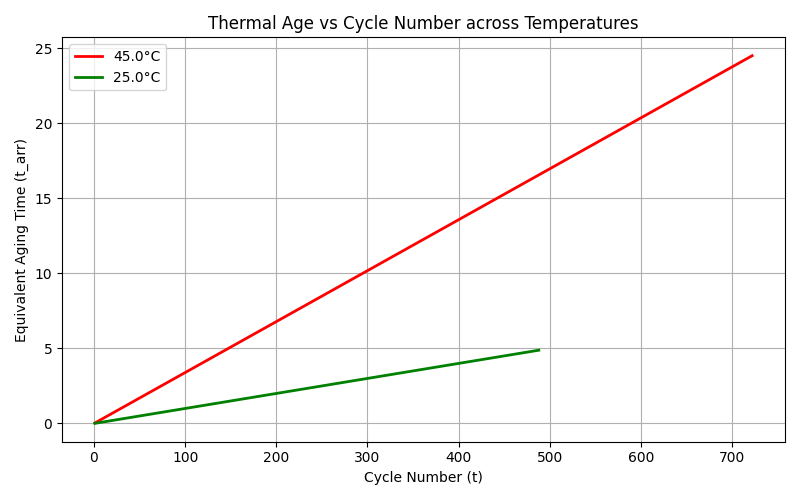
\includegraphics[width=\linewidth]{plots/plots_random_scaled/thermal_age_vs_cycle.png}
\caption{Equivalent thermal age ($t_{\text{eq}}$) versus cycle number for cells at 25\textdegree C and 45\textdegree C. The divergence reflects the learned Arrhenius scaling factor $\gamma(T)$.}
\label{fig:thermal_age}
\end{figure}

\subsection{Training Hyperparameters and Implementation}
We implemented all models in Python using the PyTorch framework. Optimization was performed over a maximum of 500 epochs using the Adam optimizer with differential learning rates: $1\times10^{-3}$ for the neural network weights and $1\times10^{-2}$ for the Arrhenius activation energy parameter ($E_a$). To dynamically adjust the optimization landscape, we used a \textit{ReduceLROnPlateau} learning rate scheduler monitored against the validation loss (\textit{mode=`min'}, \textit{factor=0.5}, \textit{patience=25}), alongside an early stopping criterion (patience of 100 epochs) to prevent overfitting.

For the training pipeline, 10\% of the data was partitioned for validation. This split was stratified by temperature for the holdout protocol and randomized for the in-distribution protocol. The parameter $E_a$ was initialized at $52.0$~kJ/mol, reflecting a typical physical value for solid electrolyte interphase (SEI) processes. Upon convergence, $E_a$ optimized to approximately $48.5$~kJ/mol on the holdout experiment and $50.5$~kJ/mol on the random split. In both cases the value remained within physically plausible bounds, validating the model's capacity to capture realistic temperature sensitivities.

\section{Results}
We evaluate both the baseline PINN (no temperature scaling) and the proposed Arrhenius PINN on two tasks: (1) in-distribution performance using a random split that mixes all temperatures (25\textdegree C, 35\textdegree C, 45\textdegree C), and (2) out-of-distribution generalization on the held-out 35\textdegree C temperature set. All metrics are computed on the original, unnormalized capacity scale (mA\textperiodcentered h) to ensure physical interpretability.

\subsection{In-Distribution Performance (Random Split)}
Table~\ref{tab:indist} compares the two models on the random split test set. The proposed Arrhenius PINN achieves a substantially lower MSE (633.19 vs. 1500.67~mA\textsuperscript{2}\textperiodcentered h\textsuperscript{2}) and a higher R\textsuperscript{2} (0.980 vs. 0.953), indicating a better overall fit. The MAE is also lower (18.40 vs. 27.42~mA\textperiodcentered h), and the RMSE improves from 38.74 to 25.16~mA\textperiodcentered h. Overall, the relative improvement in MSE is approximately 57.8\%.

\begin{table*}[!t]
\centering
\caption{In-distribution performance (random split across 25\textdegree C, 35\textdegree C, 45\textdegree C)}
\label{tab:indist}
\begin{tabular}{@{}lcccc@{}}
\toprule
Model & MSE (mA\textperiodcentered h)\textsuperscript{2} & MAE (mA\textperiodcentered h) & RMSE (mA\textperiodcentered h) & R\textsuperscript{2} \\
\midrule
Baseline PINN (no scaling) & 1500.67 & 27.42 & 38.74 & 0.953 \\
Proposed PINN (Arrhenius scaling) & \textbf{633.19} & \textbf{18.40} & \textbf{25.16} & \textbf{0.980} \\
\bottomrule
\end{tabular}
\end{table*}

\begin{table*}[!t]
\centering
\caption{Out-of-distribution performance (35\textdegree C holdout temperature)}
\label{tab:ood}
\begin{tabular}{@{}lcccc@{}}
\toprule
Model & MSE (mA\textperiodcentered h)\textsuperscript{2} & MAE (mA\textperiodcentered h) & RMSE (mA\textperiodcentered h) & R\textsuperscript{2} \\
\midrule
Baseline PINN (no scaling) & 5986.26 & 73.47 & 77.37 & $-1.760$ \\
Proposed PINN (Arrhenius scaling) & \textbf{674.26} & \textbf{21.24} & \textbf{25.97} & \textbf{0.689} \\
\bottomrule
\end{tabular}
\end{table*}

\subsection{Out-of-Distribution Generalization (35\textdegree C Holdout)}
Table~\ref{tab:ood} reports performance on the 35\textdegree C cells, which were completely unseen during training. The proposed model achieves a dramatically higher R\textsuperscript{2} (0.689 vs. $-1.760$) and a substantially lower MSE (674.26 vs. 5986.26~mA\textsuperscript{2}\textperiodcentered h\textsuperscript{2}), MAE (21.24 vs. 73.47~mA\textperiodcentered h), and RMSE (25.97 vs. 77.37~mA\textperiodcentered h). The negative R\textsuperscript{2} of the baseline indicates that, without temperature scaling, the model performs worse than simply predicting the mean SOH for the unseen temperature. In contrast, the proposed Arrhenius-scaled PINN explains 68.9\% of the variance, demonstrating that the temperature-dependent temporal scaling is essential for cross-temperature generalization.

\subsection{Qualitative SOH Trajectory Predictions}
Figures~\ref{fig:holdout_baseline} and~\ref{fig:holdout_proposed} show the predicted SOH trajectories for three representative test cells from the 35\textdegree C holdout set. The baseline PINN without scaling exhibits large deviations from the true degradation curve, while the proposed Arrhenius-scaled PINN captures the degradation trend more faithfully.

\begin{figure*}[!t]
\centering
\begin{subfigure}[b]{0.32\linewidth}
  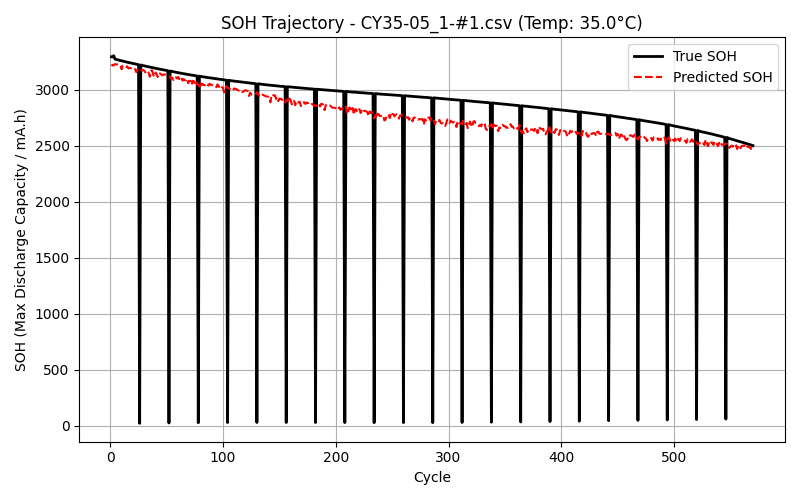
\includegraphics[width=\linewidth]{plots/plots_holdout_unscaled/soh_CY35-05_1-num1.csv.png}
  \caption{Cell 1}
\end{subfigure}
\begin{subfigure}[b]{0.32\linewidth}
  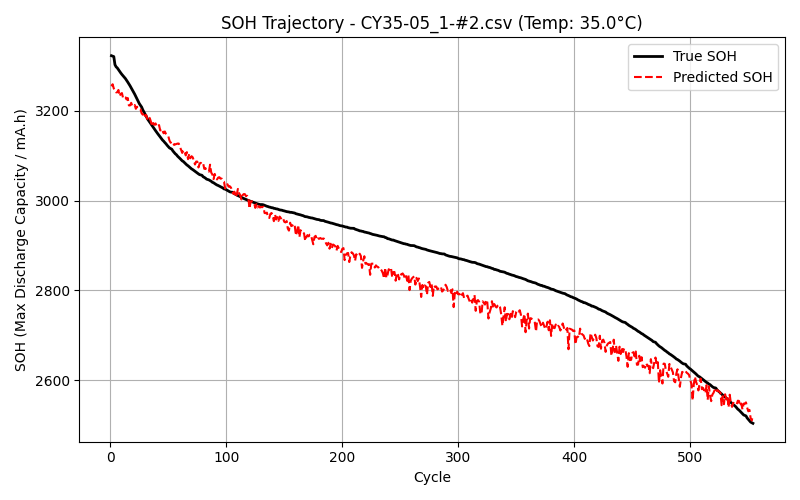
\includegraphics[width=\linewidth]{plots/plots_holdout_unscaled/soh_CY35-05_1-num2.csv.png}
  \caption{Cell 2}
\end{subfigure}
\begin{subfigure}[b]{0.32\linewidth}
  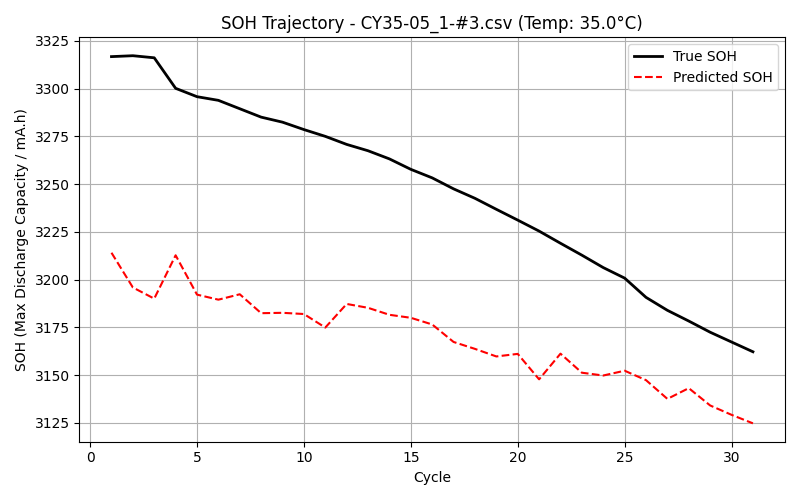
\includegraphics[width=\linewidth]{plots/plots_holdout_unscaled/soh_CY35-05_1-num3.csv.png}
  \caption{Cell 3}
\end{subfigure}
\caption{Holdout (35\textdegree C) predictions -- baseline PINN (no scaling).}
\label{fig:holdout_baseline}
\end{figure*}

\begin{figure*}[!t]
\centering
\begin{subfigure}[b]{0.32\linewidth}
  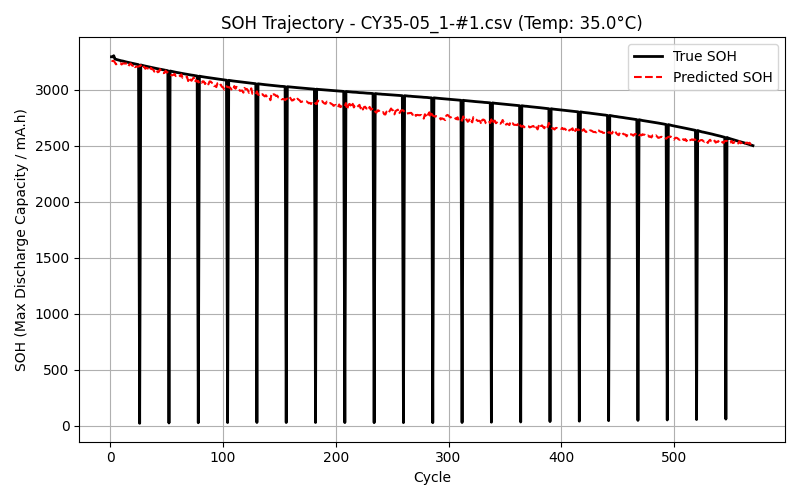
\includegraphics[width=\linewidth]{plots/plots_holdout_scaled/soh_CY35-05_1-num1.csv.png}
  \caption{Cell 1}
\end{subfigure}
\begin{subfigure}[b]{0.32\linewidth}
  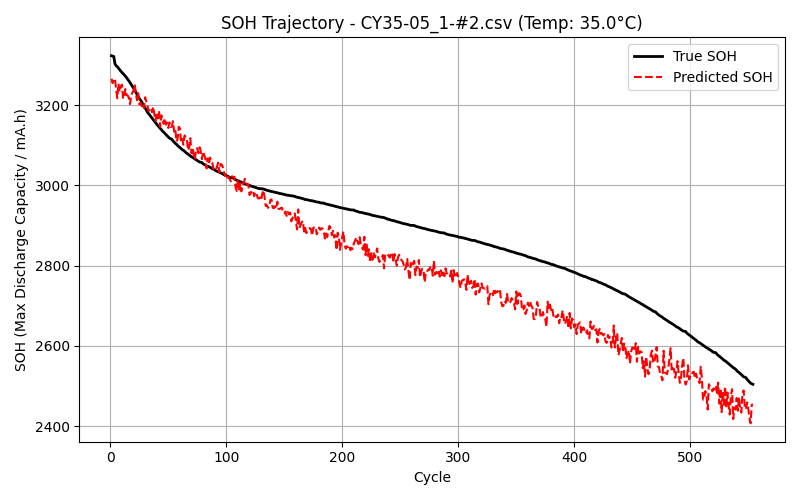
\includegraphics[width=\linewidth]{plots/plots_holdout_scaled/soh_CY35-05_1-num2.csv.png}
  \caption{Cell 2}
\end{subfigure}
\begin{subfigure}[b]{0.32\linewidth}
  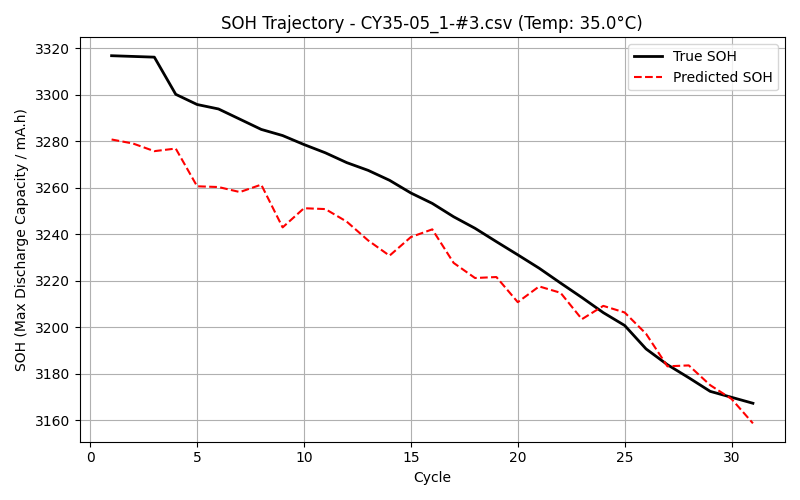
\includegraphics[width=\linewidth]{plots/plots_holdout_scaled/soh_CY35-05_1-num3.csv.png}
  \caption{Cell 3}
\end{subfigure}
\caption{Holdout (35\textdegree C) predictions -- proposed Arrhenius-scaled PINN.}
\label{fig:holdout_proposed}
\end{figure*}

Figures~\ref{fig:random_baseline} and~\ref{fig:random_proposed} show four representative test cells from the random split (in-distribution), covering cells at 25\textdegree C and 45\textdegree C. The proposed model consistently tracks the true SOH more accurately, with less deviation in both early and late cycles.

\begin{figure*}[!t]
\centering
\begin{subfigure}[b]{0.48\linewidth}
  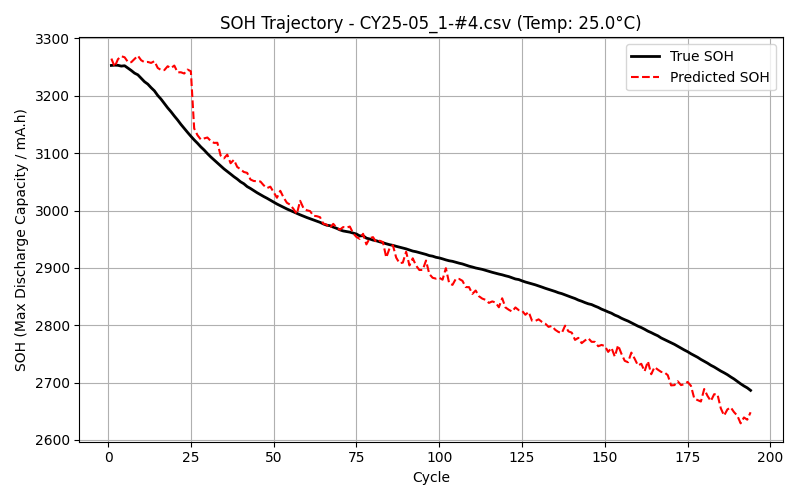
\includegraphics[width=\linewidth]{plots/plots_random_unscaled/soh_CY25-05_1-num4.csv.png}
  \caption{CY25-05 Cell 4 (25\textdegree C)}
\end{subfigure}
\begin{subfigure}[b]{0.48\linewidth}
  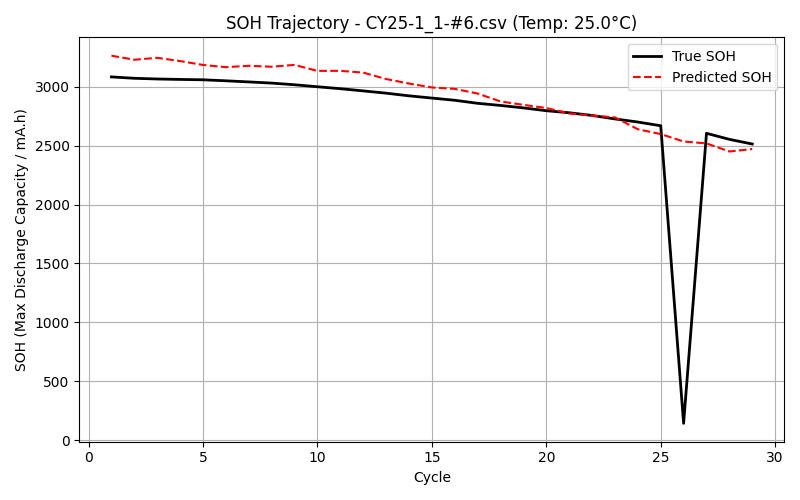
\includegraphics[width=\linewidth]{plots/plots_random_unscaled/soh_CY25-1_1-num6.csv.png}
  \caption{CY25-1 Cell 6 (25\textdegree C)}
\end{subfigure}
\begin{subfigure}[b]{0.48\linewidth}
  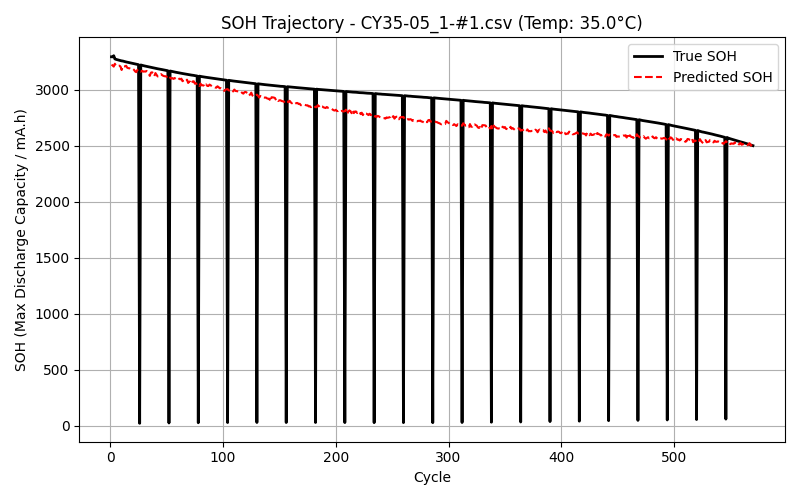
\includegraphics[width=\linewidth]{plots/plots_random_unscaled/soh_CY35-05_1-num1.csv.png}
  \caption{CY35-05 Cell 1 (35\textdegree C)}
\end{subfigure}
\begin{subfigure}[b]{0.48\linewidth}
  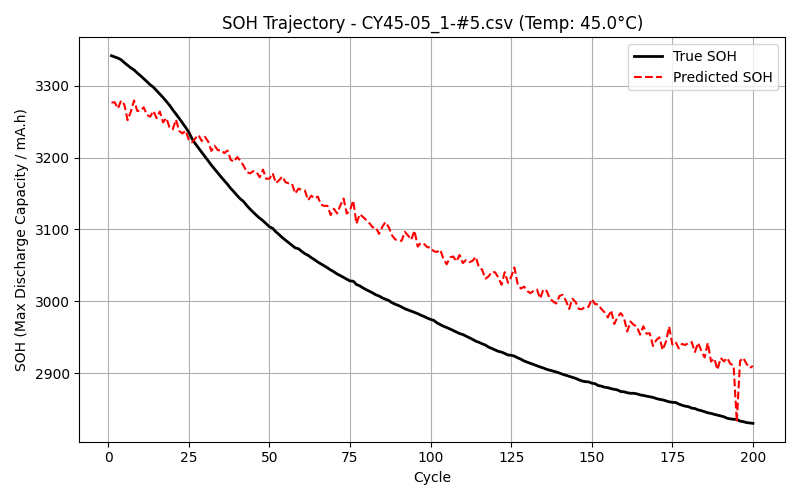
\includegraphics[width=\linewidth]{plots/plots_random_unscaled/soh_CY45-05_1-num5.csv.png}
  \caption{CY45-05 Cell 5 (45\textdegree C)}
\end{subfigure}
\caption{Random split (in-distribution) predictions -- baseline PINN (no scaling).}
\label{fig:random_baseline}
\end{figure*}

\begin{figure*}[!t]
\centering
\begin{subfigure}[b]{0.48\linewidth}
  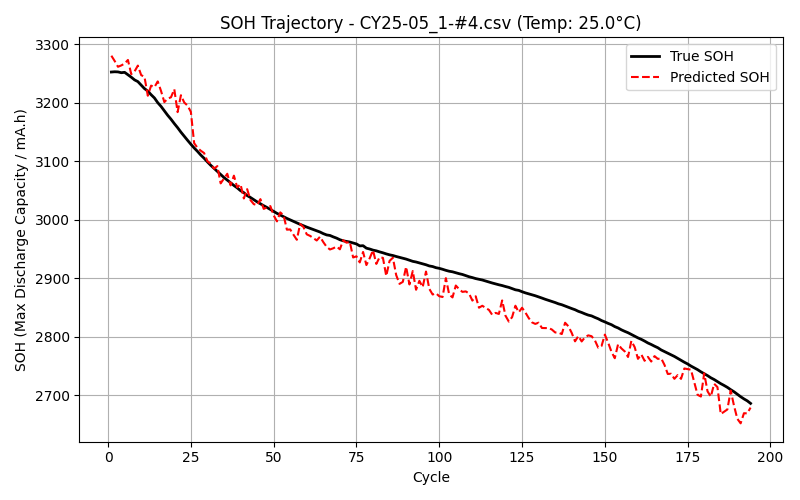
\includegraphics[width=\linewidth]{plots/plots_random_scaled/soh_CY25-05_1-num4.csv.png}
  \caption{CY25-05 Cell 4 (25\textdegree C)}
\end{subfigure}
\begin{subfigure}[b]{0.48\linewidth}
  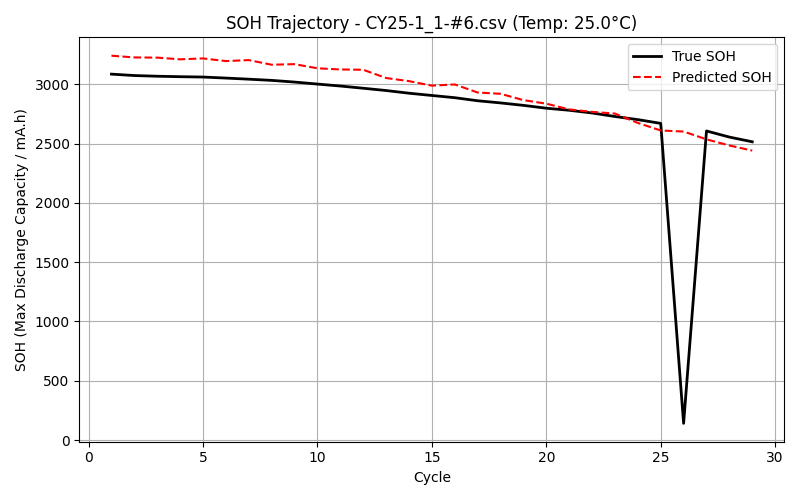
\includegraphics[width=\linewidth]{plots/plots_random_scaled/soh_CY25-1_1-num6.csv.png}
  \caption{CY25-1 Cell 6 (25\textdegree C)}
\end{subfigure}
\begin{subfigure}[b]{0.48\linewidth}
  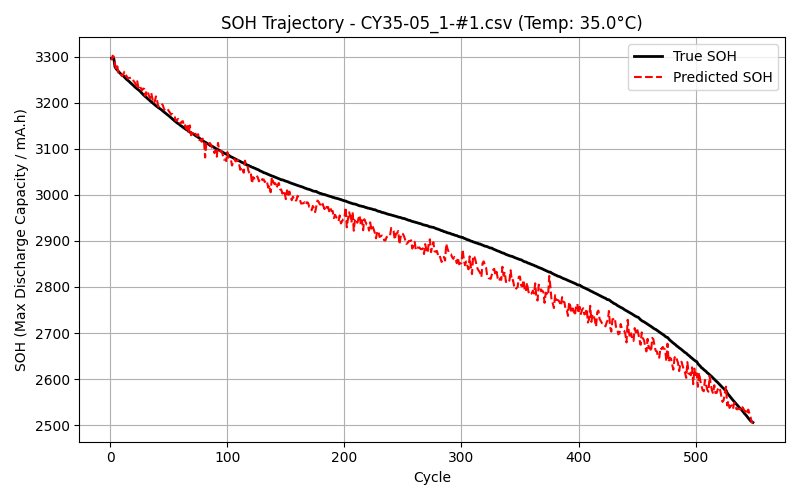
\includegraphics[width=\linewidth]{plots/plots_random_scaled/soh_CY35-05_1-num1.csv.png}
  \caption{CY35-05 Cell 1 (35\textdegree C)}
\end{subfigure}
\begin{subfigure}[b]{0.48\linewidth}
  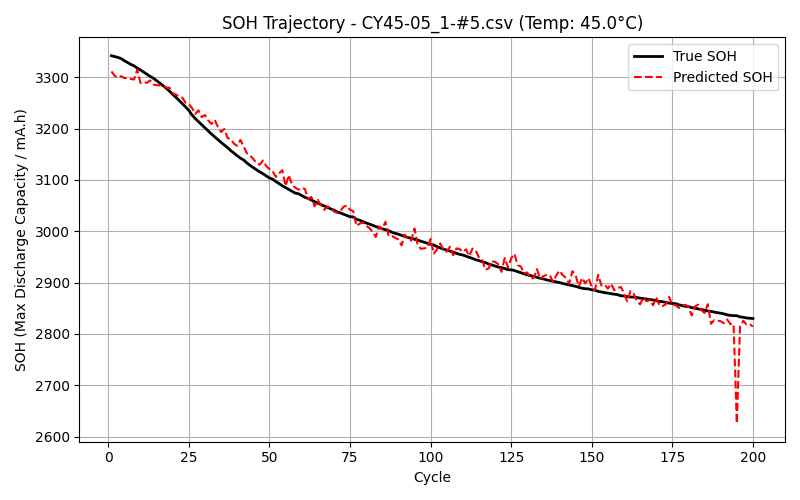
\includegraphics[width=\linewidth]{plots/plots_random_scaled/soh_CY45-05_1-num5.csv.png}
  \caption{CY45-05 Cell 5 (45\textdegree C)}
\end{subfigure}
\caption{Random split (in-distribution) predictions -- proposed Arrhenius-scaled PINN.}
\label{fig:random_proposed}
\end{figure*}

\section{Conclusion}
We have presented a simple yet physically meaningful enhancement to the battery PINN framework: replacing raw cycle number with an Arrhenius-scaled equivalent aging time, where the activation energy is treated as a learnable parameter. This modification embeds the well-known temperature acceleration of battery degradation directly into the model's temporal coordinate. On the TJU NCA dataset, the proposed method substantially improves both in-distribution and out-of-distribution performance. For the in-distribution random split, R\textsuperscript{2} increases from 0.953 to 0.980 while MSE decreases from 1500.67 to 633.19~mA\textsuperscript{2}\textperiodcentered h\textsuperscript{2}. For the challenging out-of-distribution 35\textdegree C holdout test, the proposed model improves R\textsuperscript{2} from $-1.760$ to $0.689$ and reduces RMSE from 77.37 to 25.97~mA\textperiodcentered h, an improvement of 66.4\%. The learned activation energy converges to approximately 48.5--50.5~kJ/mol, which is physically plausible and consistent with reported SEI-growth kinetics.

\section{Code Availability}
The source code used in this work is publicly available at:
\url{https://github.com/Sel68/temp-scaled-PINN-SOH}

\newpage
\FloatBarrier
\begin{thebibliography}{00}
\bibitem{wang2024physics}
F. Wang, Z. Zhao, Y. Di, and X. Chen, ``Physics-informed neural network for lithium-ion battery degradation stable modeling and prognosis,'' \textit{Nat. Commun.}, vol. 15, p. 4332, 2024.
\bibitem{spotnitz2003}
R. Spotnitz, ``Simulation of capacity fade in lithium-ion batteries,'' \textit{J. Power Sources}, vol. 113, no. 1, pp. 72--80, 2003.
\bibitem{bloom2005}
I. Bloom, B. W. Cole, J. J. Sohn, S. A. Jones, E. G. Polzin, V. S. Battaglia, G. L. Henriksen, C. Motloch, R. Richardson, T. Unkelhaeuser, and D. Ingersoll, ``An accelerated calendar and cycle life study of Li-ion cells,'' \textit{J. Power Sources}, vol. 139, no. 1--2, pp. 295--303, 2005.
\bibitem{severson2019}
K. A. Severson, P. M. Attia, N. Jin, N. Perkins, B. Jiang, Z. Yang, M. H. Chen, M. Aykol, P. K. Herring, D. Fraggedakis, and others, ``Data-driven prediction of battery cycle life before capacity degradation,'' \textit{Nature Energy}, vol. 4, no. 5, pp. 383--391, 2019.
\bibitem{raissi2019physics}
M. Raissi, P. Perdikaris, and G. E. Karniadakis, ``Physics-informed neural networks: A deep learning framework for solving forward and inverse problems involving nonlinear partial differential equations,'' \textit{J. Comput. Phys.}, vol. 378, pp. 686--707, 2019.
\bibitem{zhu2022data}
J. Zhu, Y. Wang, Y. Huang, R. B. Gopaluni, Y. Cao, M. Heere, M. J. M\"{u}hlbauer, L. Mereacre, H. Dai, X. Liu, and others, ``Data-driven capacity estimation of commercial lithium-ion batteries from voltage relaxation,'' \textit{Nat. Commun.}, vol. 13, p. 2261, 2022.
\end{thebibliography}

\end{document}